\documentclass[aspectratio=169, table]{beamer}

\usepackage{colortbl}
\usepackage{xcolor}
\usepackage{listings}
\usepackage{pgfplots}
\usepgfplotslibrary{polar}
\pgfplotsset{compat=1.18}
\usepackage{tikz}
\usetikzlibrary{shapes.geometric,
	positioning, shapes, shapes.multipart, backgrounds, arrows.meta, calc, fit, trees}

\makeatletter
\def\input@path{{../theme/}}
\makeatother
\graphicspath{{../theme/}}
\usetheme{Pradita}

\lstdefinelanguage{xml}{
	keywords={},
	basicstyle=\ttfamily\scriptsize,
	keywordstyle=\color{blue}\bfseries,
	sensitive=true,
	commentstyle=\color{gray}\ttfamily,
	stringstyle=\color{purple}\ttfamily,
	numbers=left,
	numberstyle=\tiny\color{gray},
	breaklines=true,
	frame=lines,
	backgroundcolor=\color{lightgray!10},
	tabsize=2,
	morecomment=[s]{<!--}{-->},
	morestring=[b]",
	morestring=[b]',
	showstringspaces=false
}

\lstdefinelanguage{json}{
	keywords={true,false,null},
	keywordstyle=\color{blue}\bfseries,
	sensitive=true,
	comment=[l]{//},
	commentstyle=\color{gray}\ttfamily\itshape,
	stringstyle=\color{purple}\ttfamily,
	morestring=[b]",
	basicstyle=\ttfamily\scriptsize,
	numbers=left,
	numberstyle=\tiny\color{gray},
	breaklines=true,
	frame=lines,
	backgroundcolor=\color{lightgray!10},
	showstringspaces=false
}

\lstdefinelanguage{java}{
  keywords={package,import,public,class,interface,extends,implements,
            return,new,null,true,false,void,if,else,for,while,static,
            final,private,protected,String,throws,Exception,try,finally},
  keywordstyle=\color{blue}\bfseries,
  sensitive=true,
  comment=[l]{//},
  morecomment=[s]{/*}{*/},
  commentstyle=\color{gray}\ttfamily\itshape,
  stringstyle=\color{purple}\ttfamily,
  morestring=[b]",
  basicstyle=\ttfamily\scriptsize,
  numbers=left,
  numberstyle=\tiny\color{gray},
  breaklines=true,
  frame=lines,
  backgroundcolor=\color{lightgray!10},
  showstringspaces=false
}

\lstdefinelanguage{egx}{
  keywords={rule,transform,parameters,template,target,pre,post,var,Map},
  keywordstyle=\color{blue}\bfseries,
  sensitive=true,
  comment=[l]{//},
  morecomment=[s]{/*}{*/},
  commentstyle=\color{gray}\ttfamily\itshape,
  stringstyle=\color{purple}\ttfamily,
  morestring=[b]",
  basicstyle=\ttfamily\scriptsize,
  numbers=left,
  numberstyle=\tiny\color{gray},
  breaklines=true,
  frame=lines,
  backgroundcolor=\color{lightgray!10},
  showstringspaces=false
}

\lstdefinelanguage{eol}{
  keywords={operation,return,if,else,var,while,for,in,not,and,or,new,self,true,false,null,import},
  keywordstyle=\color{blue}\bfseries,
  sensitive=true,
  comment=[l]{//},
  morecomment=[s]{/*}{*/},
  commentstyle=\color{gray}\ttfamily\itshape,
  stringstyle=\color{purple}\ttfamily,
  morestring=[b]",
  basicstyle=\ttfamily\scriptsize,
  numbers=left,
  numberstyle=\tiny\color{gray},
  breaklines=true,
  frame=lines,
  backgroundcolor=\color{lightgray!10},
  showstringspaces=false
}

\lstdefinelanguage{egl}{
  keywords={import,var,for,in,if,else,not,and,or,return,operation,Any,String,Integer,Sequence,Boolean,Real},
  keywordstyle=\color{blue}\bfseries,
  sensitive=true,
  comment=[l]{//},
  morecomment=[s]{/*}{*/},
  commentstyle=\color{gray}\ttfamily\itshape,
  stringstyle=\color{purple}\ttfamily,
  morestring=[b]",
  basicstyle=\ttfamily\scriptsize,
  numbers=left,
  numberstyle=\tiny\color{gray},
  breaklines=true,
  frame=lines,
  backgroundcolor=\color{lightgray!10},
  showstringspaces=false,
  moredelim=**[is][\color{red}\bfseries]{[\%}{\%]}
}

\lstdefinelanguage{javascript}{
  keywords={const,let,var,async,await,function,return,if,for,of,true,false,null},
  keywordstyle=\color{blue}\bfseries,
  sensitive=true,
  comment=[l]{//},
  morecomment=[s]{/*}{*/},
  commentstyle=\color{gray}\ttfamily\itshape,
  stringstyle=\color{purple}\ttfamily,
  morestring=[b]",
  morestring=[b]`,
  basicstyle=\ttfamily\scriptsize,
  numbers=left,
  numberstyle=\tiny\color{gray},
  breaklines=true,
  frame=lines,
  backgroundcolor=\color{lightgray!10},
  showstringspaces=false
}

\subtitle{IT30213 - Advanced Software Engineering \& DevOps}
\title{\Huge Model-to-Text\vspace{8pt}\\Transformation}
\author{\textbf{Alfa Yohannis}}

\begin{document}

\frame{\titlepage}

\begin{frame}[fragile]
	\frametitle{Contents}
	\vspace{20pt}
	\begin{columns}[t]
		\column{0.5\textwidth}
		\tableofcontents[sections={1-4}]

		\column{0.5\textwidth}
		\tableofcontents[sections={5-8}]
	\end{columns}
\end{frame}

\begin{frame}{\hfill}
	\centering
	\Huge{\textbf{Bagaimana menghasilkan kode program atau dokumentasi dari model abstrak yang sudah kita bangun?}}
\end{frame}

% ============================================================
\section{Tujuan Pembelajaran}
\begin{frame}{\hfill}
	\centering
	\Huge{\textbf{Tujuan Pembelajaran}}
\end{frame}

\begin{frame}{Tujuan Pembelajaran}
\vspace{6pt}
Setelah sesi ini, mahasiswa diharapkan mampu:
\begin{enumerate}
  \item Menjelaskan peran transformasi model-ke-teks (M2T) dalam siklus \textit{Model-Driven Engineering}.
  \item Membedakan tanggung jawab EGL, EGX, dan EOL dalam implementasi transformasi M2T.
  \item Menerapkan M2T pada model \textit{MediaFlow} untuk menghasilkan JSON ELK dan fragmen HTML, sekaligus menganalisis isu identifier, escaping, referensi port-ke-node, dan validasi output.
\end{enumerate}
\end{frame}

% ============================================================
\section{Pendahuluan}
\begin{frame}{\hfill}
	\centering
	\Huge{\textbf{Pendahuluan}}
\end{frame}

\begin{frame}{M2M vs M2T}
\vspace{6pt}
\begin{columns}[T]
\column{0.5\textwidth}
\textbf{Model-to-Model (M2M)}
\begin{itemize}
  \item Input: model sumber.
  \item Output: model target.
  \item Output tetap berkonformasi ke metamodel.
  \item Contoh sesi 11: \textit{MediaFlow} menjadi UML Activity Diagram.
\end{itemize}

\column{0.5\textwidth}
\textbf{Model-to-Text (M2T)}
\begin{itemize}
  \item Input: model sumber.
  \item Output: artefak teks.
  \item Output dikonsumsi oleh parser, compiler, browser, atau runtime.
  \item Contoh sesi 12: \textit{MediaFlow} menjadi JSON ELK dan HTML.
\end{itemize}
\end{columns}
\end{frame}

\begin{frame}{Posisi M2T dalam MDE}
\vspace{6pt}
\centering
\scalebox{0.85}{
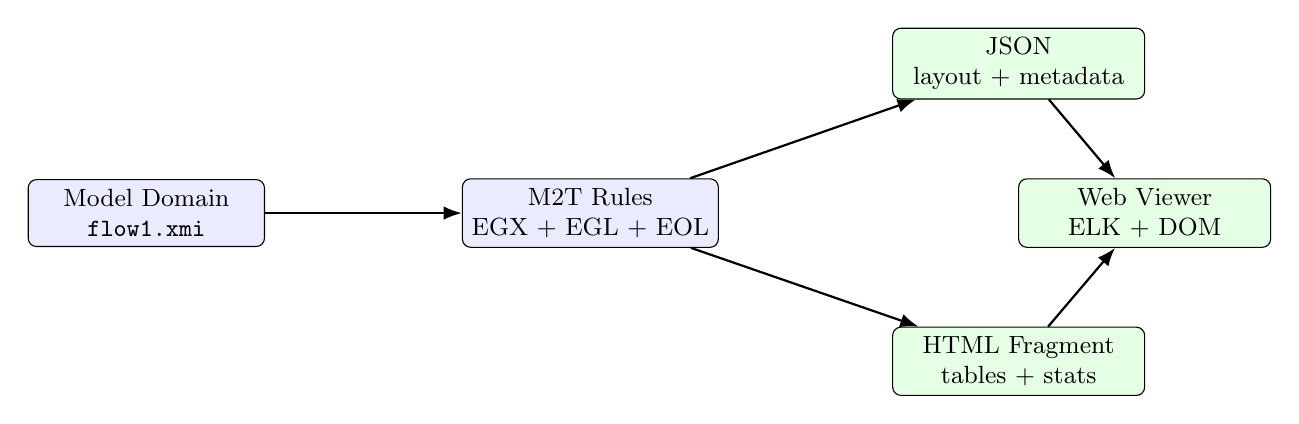
\begin{tikzpicture}[>=Latex, node distance=14mm,
  box/.style={draw, rounded corners=3pt, minimum width=3.0cm, minimum height=0.85cm, align=center, fill=blue!8, font=\small},
  target/.style={draw, rounded corners=3pt, minimum width=3.2cm, minimum height=0.85cm, align=center, fill=green!10, font=\small}]
  \node[box] (model) {Model Domain\\\texttt{flow1.xmi}};
  \node[box, right=25mm of model] (m2t) {M2T Rules\\EGX + EGL + EOL};
  \node[target, above right=10mm and 22mm of m2t] (json) {JSON\\layout + metadata};
  \node[target, below right=10mm and 22mm of m2t] (html) {HTML Fragment\\tables + stats};
  \node[target, right=38mm of m2t] (viewer) {Web Viewer\\ELK + DOM};

  \draw[->, thick] (model) -- (m2t);
  \draw[->, thick] (m2t) -- (json);
  \draw[->, thick] (m2t) -- (html);
  \draw[->, thick] (json) -- (viewer);
  \draw[->, thick] (html) -- (viewer);
\end{tikzpicture}
}

\vspace{8pt}
\small
M2T adalah titik ketika model berubah menjadi artefak teknis: teks harus benar secara semantik \textit{dan} valid secara leksikal.
\end{frame}

% ============================================================
\section{Masalah Domain}
\begin{frame}{\hfill}
	\centering
	\Huge{\textbf{Masalah Domain}}
\end{frame}

\begin{frame}{Studi Kasus: Mediaflow Viewer}
\vspace{6pt}
\begin{columns}[T]
\column{0.48\textwidth}
\textbf{Domain Sumber}
\begin{itemize}
  \item \texttt{Graph} sebagai kontainer.
  \item \texttt{Node}: \texttt{Resource}, \texttt{Scaler}, \texttt{Transcoder}.
  \item \texttt{Port}: arah \texttt{IN}/\texttt{OUT}.
  \item \texttt{Edge}: menghubungkan port sumber ke port target.
\end{itemize}

\column{0.52\textwidth}
\textbf{Korpus Input}
\begin{itemize}
  \item \texttt{flow1.xmi}: pipeline linier, 3 node, 2 edge.
  \item \texttt{flow2.xmi}: pipeline bercabang, 6 node, 5 edge.
  \item Atribut penting: \texttt{command}, \texttt{backend}, \texttt{width}, \texttt{height}, \texttt{videoCodec}, \texttt{bitrate}.
\end{itemize}
\end{columns}

\vspace{8pt}
\textbf{Masalah:} browser viewer tidak ideal membaca XMI mentah. Model perlu diturunkan menjadi format web yang lebih langsung.
\end{frame}

\begin{frame}{Target Transformasi}
\vspace{6pt}
\begin{columns}[T]
\column{0.5\textwidth}
\textbf{1. JSON ELK}
\begin{itemize}
  \item Lokasi: \texttt{output/elk/}\\\texttt{<graph.name>.json}.
  \item Struktur untuk \texttt{ELK.layout()}.
  \item Memuat \texttt{children}, \texttt{ports}, \texttt{edges}, dan \texttt{layoutOptions}.
  \item Memuat \texttt{nodeMeta} dan \texttt{edgeMeta} untuk tooltip.
\end{itemize}

\column{0.5\textwidth}
\textbf{2. HTML Fragment}
\begin{itemize}
  \item Lokasi: \texttt{output/tables/}\\\texttt{<graph.name>.tables.html}.
  \item Bukan halaman penuh.
  \item Disisipkan ke panel samping viewer.
  \item Memuat statistik, tabel node, dan tabel edge.
\end{itemize}
\end{columns}
\end{frame}

\begin{frame}{Pemetaan Konseptual}
\vspace{2pt}
\tiny
\begin{tabular}{|p{0.18\textwidth}|p{0.37\textwidth}|p{0.35\textwidth}|}
\hline
\rowcolor{black!8}
\textbf{MediaFlow} & \textbf{JSON ELK} & \textbf{HTML Fragment} \\
\hline
\texttt{Graph} & Root: \texttt{name}, \texttt{elk}, \texttt{nodeMeta}, \texttt{edgeMeta}. & Section \texttt{data-flow}. \\
\hline
\texttt{Node} & \texttt{child}: id, label, ukuran, port. & Baris tabel node. \\
\hline
\texttt{Port} & Id stabil; \texttt{OUT} ke \texttt{EAST}, lainnya ke \texttt{WEST}. & Statistik port masuk/keluar. \\
\hline
\texttt{Edge} & Edge dari id port sumber ke id port target. & Baris tabel edge. \\
\hline
\texttt{Resource} & \texttt{uri}, \texttt{external}, \texttt{mediaType}. & Hitungan resource/external. \\
\hline
\texttt{Scaler} & \texttt{backend}, \texttt{command}, \texttt{width}, \texttt{height}. & Hitungan scaler. \\
\hline
\texttt{Transcoder} & Codec, container, bitrate, command. & Hitungan transcoder. \\
\hline
\end{tabular}
\end{frame}

% ============================================================
\section{Arsitektur M2T}
\begin{frame}{\hfill}
	\centering
	\Huge{\textbf{Arsitektur M2T}}
\end{frame}

\begin{frame}{Pipeline Proyek \texttt{m2t}}
\vspace{4pt}
\centering
\scalebox{.95}{
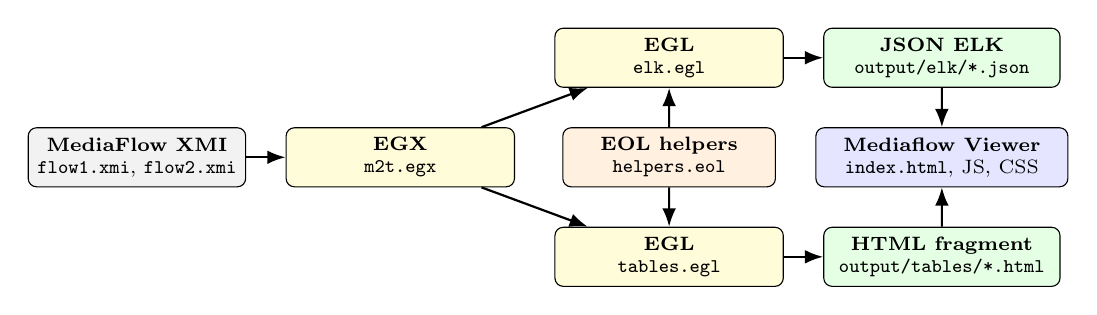
\begin{tikzpicture}[>=Latex, node distance=0mm,
  box/.style={draw, rounded corners=3pt, minimum width=2.7cm, minimum height=0.75cm, align=center, font=\scriptsize},
  artifact/.style={draw, rounded corners=3pt, minimum width=3.0cm, minimum height=0.75cm, align=center, font=\scriptsize, fill=green!10},
  engine/.style={draw, rounded corners=3pt, minimum width=2.9cm, minimum height=0.75cm, align=center, font=\scriptsize, fill=yellow!15},
  viewer/.style={draw, rounded corners=3pt, minimum width=3.2cm, minimum height=0.75cm, align=center, font=\scriptsize, fill=blue!10}]

  \node[box, fill=gray!10] (xmi) {\textbf{MediaFlow XMI}\\\texttt{flow1.xmi}, \texttt{flow2.xmi}};

  \node[engine, right=5mm of xmi] (egx) {\textbf{EGX}\\\texttt{m2t.egx}};

  \node[engine, above right=5mm and 5mm of egx] (egl1) {\textbf{EGL}\\\texttt{elk.egl}};

  \node[engine, below right=5mm and 5mm of egx] (egl2) {\textbf{EGL}\\\texttt{tables.egl}};

  \node[box, right=6mm of egx, fill=orange!12] (eol) {\textbf{EOL helpers}\\\texttt{helpers.eol}};

  \node[artifact, right=5mm of egl1] (json) {\textbf{JSON ELK}\\\texttt{output/elk/*.json}};

  \node[artifact, right=5mm of egl2] (html) {\textbf{HTML fragment}\\\texttt{output/tables/*.html}};
  
  \node[viewer, right=5mm of eol] (web) {\textbf{Mediaflow Viewer}\\\texttt{index.html}, JS, CSS};

  \draw[->, thick] (xmi) -- (egx);
  \draw[->, thick] (egx) -- (egl1);
  \draw[->, thick] (egx) -- (egl2);
  \draw[->, thick] (eol) -- (egl1);
  \draw[->, thick] (eol) -- (egl2);
  \draw[->, thick] (egl1) -- (json);
  \draw[->, thick] (egl2) -- (html);
  \draw[->, thick] (json) -- (web);
  \draw[->, thick] (html) -- (web);
\end{tikzpicture}
}
\vspace{6pt}
\small
EGX mengorkestrasi file; EGL menulis teks; EOL menjaga logika bantuan tetap modular.
\end{frame}

\begin{frame}[fragile]{Struktur Proyek}
\vspace{2pt}
\begin{columns}[T,onlytextwidth]
\column{0.66\textwidth}
\begin{lstlisting}[basicstyle=\ttfamily\tiny, breaklines=true]
m2t/
|-- src/m2t/
|   +-- MediaflowToHtmlEGXRunner.java
|-- transformer/
|   |-- m2t.egx
|   |-- elk.egl
|   |-- tables.egl
|   +-- helpers.eol
|-- input/
|   |-- flow1.xmi
|   +-- flow2.xmi
|-- output/
|   |-- manifest.json
|   |-- index.html
|   |-- css/style.css
|   |-- js/app.js
|   |-- elk/flow1.json
|   |-- elk/flow2.json
|   |-- tables/flow1.tables.html
|   +-- tables/flow2.tables.html
\end{lstlisting}

\column{0.31\textwidth}
\scriptsize
\textbf{Penjelasan singkat}
\begin{itemize}
  \item \texttt{src/}: runner Java.
  \item \texttt{transformer/}: aturan dan template.
  \item \texttt{input/}: model XMI.
  \item \texttt{output/}: artefak web hasil M2T.
  \item Metamodel tetap dirujuk dari proyek \texttt{mediaflow}.
\end{itemize}
\end{columns}
\end{frame}

% ============================================================
\section{Implementasi Epsilon}
\begin{frame}{\hfill}
	\centering
	\Huge{\textbf{Implementasi Epsilon}}
\end{frame}

\begin{frame}[fragile]{Koordinator EGX: Dua Output per Graph}
\vspace{2pt}
\begin{columns}[T,onlytextwidth]
\column{0.66\textwidth}
\begin{lstlisting}[language=egx, basicstyle=\ttfamily\tiny]
rule Graph2ElkJson
    transform graph : Mediaflow!Graph {

    parameters : Map { "graph" = graph }
    template : "elk.egl"
    target : "../output/elk/" + graph.name + ".json"
}

rule Graph2Tables
    transform graph : Mediaflow!Graph {

    parameters : Map { "graph" = graph }
    template : "tables.egl"
    target : "../output/tables/" + graph.name + ".tables.html"
}
\end{lstlisting}

\column{0.31\textwidth}
\scriptsize
\textbf{Penjelasan singkat}
\begin{itemize}
  \item Satu \texttt{Graph} diproses dua kali.
  \item \texttt{parameters} mengirim objek model ke EGL.
  \item \texttt{template} memilih file pembangkit teks.
  \item \texttt{target} menentukan lokasi output.
\end{itemize}
\end{columns}
\end{frame}

\begin{frame}[fragile]{Helper EOL: Escaping dan Navigasi Model}
\vspace{2pt}
\begin{columns}[T,onlytextwidth]
\column{0.66\textwidth}
\begin{lstlisting}[language=eol, basicstyle=\ttfamily\tiny]
operation Any jsonValue() : String {
    if (self == null) { return "null"; }
    if (self.isKindOf(Boolean)) { return self.asString(); }
    if (self.isKindOf(Integer) or self.isKindOf(Real)) {
        return self.asString();
    }
    return "\"" + self.jsonEscape() + "\"";
}

operation Mediaflow!Port isOut() : Boolean {
    return self.direction.toString() == "OUT";
}

operation Mediaflow!Edge sourceNode() : Mediaflow!Node {
    return Mediaflow!Node.all.selectOne(n | n.ports.includes(self.source));
}

operation Mediaflow!Edge targetNode() : Mediaflow!Node {
    return Mediaflow!Node.all.selectOne(n | n.ports.includes(self.target));
}
\end{lstlisting}

\column{0.31\textwidth}
\scriptsize
\textbf{Penjelasan singkat}
\begin{itemize}
  \item \texttt{jsonValue()} menjaga nilai valid sebagai JSON.
  \item \texttt{isOut()} menentukan sisi port.
  \item \texttt{sourceNode()} dan \texttt{targetNode()} menyelesaikan referensi port-ke-node.
  \item Helper dipakai ulang oleh beberapa template.
\end{itemize}
\end{columns}
\end{frame}

\begin{frame}[fragile]{EGL: Membentuk Identifier Stabil}
\vspace{2pt}
\begin{columns}[T,onlytextwidth]
\column{0.66\textwidth}
\begin{lstlisting}[language=egl, basicstyle=\ttfamily\tiny]
[%
import "helpers.eol";

var nodes = graph.nodes;
var edges = graph.edges;

var nodeIdx = new Map;
var portIdx = new Map;

var i = 0;
for (n in nodes) {
    nodeIdx.put(n, "n" + i);
    var j = 0;
    for (p in n.ports) {
        portIdx.put(p, "n" + i + "_p" + j);
        j = j + 1;
    }
    i = i + 1;
}
%]
\end{lstlisting}

\column{0.31\textwidth}
\scriptsize
\textbf{Penjelasan singkat}
\begin{itemize}
  \item \texttt{import} memuat helper EOL.
  \item \texttt{nodeIdx} memetakan node ke id.
  \item \texttt{portIdx} memetakan port ke id.
  \item Id stabil dipakai oleh layout, tooltip, dan tabel.
\end{itemize}
\end{columns}
\end{frame}

\begin{frame}[fragile]{EGL: Skeleton Output JSON}
\vspace{2pt}
\begin{columns}[T,onlytextwidth]
\column{0.66\textwidth}
\begin{lstlisting}[language=egl, basicstyle=\ttfamily\tiny]
{
  "name": "[%=graph.name.jsonEscape()%]",
  "elk": {
    "id": "root",
    "layoutOptions": {
      "elk.algorithm": "layered",
      "elk.direction": "RIGHT",
      "elk.portConstraints": "FIXED_ORDER"
    },
    "children": [
    [%=nodeJson%]
    ],
    "edges": [
    [%=edgeJson%]
    ]
  },
  "nodeMeta": { [%=metaJson%] },
  "edgeMeta": { [%=edgeMetaJson%] }
}
\end{lstlisting}

\column{0.31\textwidth}
\scriptsize
\textbf{Penjelasan singkat}
\begin{itemize}
  \item \texttt{name} berasal dari model.
  \item \texttt{elk} adalah input untuk \texttt{ELK.layout()}.
  \item \texttt{children} berisi node.
  \item \texttt{edges} berisi koneksi port.
  \item Metadata dipakai viewer untuk detail tambahan.
\end{itemize}
\end{columns}
\end{frame}

\begin{frame}[fragile]{EGL: Fragmen HTML untuk Panel Data}
\vspace{2pt}
\begin{columns}[T,onlytextwidth]
\column{0.66\textwidth}
\begin{lstlisting}[language=egl, basicstyle=\ttfamily\tiny]
<section class="fragment" data-flow="[%=graph.name%]">
  <header class="frag-head">
    <h2>[%=graph.name%]</h2>
  </header>

  <div class="stats">
    <div class="stat-group">
      <h3>Overview</h3>
      <table>
        <tr><td>Nodes</td><td class="v">[%=nodeCount%]</td></tr>
        <tr><td>Edges</td><td class="v">[%=edgeCount%]</td></tr>
        <tr><td>Ports</td><td class="v">[%=portCount%]</td></tr>
      </table>
    </div>
  </div>

  <h3>Nodes</h3>
  <table class="grid"><tbody>[%=nodeRows%]</tbody></table>
</section>
\end{lstlisting}

\column{0.31\textwidth}
\scriptsize
\textbf{Penjelasan singkat}
\begin{itemize}
  \item Satu fragmen untuk satu \texttt{Graph}.
  \item \texttt{data-flow} mengikat fragmen ke nama flow.
  \item Statistik memberi ringkasan cepat.
  \item \texttt{nodeRows} adalah baris tabel yang sudah digenerasi.
\end{itemize}
\end{columns}
\end{frame}

% ============================================================
\section{Runner dan Viewer}
\begin{frame}{\hfill}
	\centering
	\Huge{\textbf{Runner dan Viewer}}
\end{frame}

\begin{frame}[fragile]{Runner Java: Memuat Model dan Menjalankan EGX}
\vspace{2pt}
\begin{columns}[T,onlytextwidth]
\column{0.66\textwidth}
\begin{lstlisting}[language=java, basicstyle=\ttfamily\tiny]
EmfModel model = new EmfModel();
model.setName("Mediaflow");
model.setMetamodelFile(new File(metamodelPath).getAbsolutePath());
model.setModelFile(input.toAbsolutePath().toString());
model.setReadOnLoad(true);
model.setStoredOnDisposal(false);
model.load();

EglFileGeneratingTemplateFactory factory =
    new EglFileGeneratingTemplateFactory();
factory.setOutputRoot(new File(egxPath).getAbsoluteFile().getParent());

EgxModule module = new EgxModule(factory);
try {
    module.parse(new File(egxPath));
    module.getContext().getModelRepository().addModel(model);
    module.execute();
} finally {
    module.getContext().getModelRepository().dispose();
    module.getContext().dispose();
}
\end{lstlisting}

\column{0.31\textwidth}
\scriptsize
\textbf{Penjelasan singkat}
\begin{itemize}
  \item \texttt{EmfModel} memuat XMI sumber.
  \item Model hanya dibaca, tidak disimpan ulang.
  \item Factory menentukan root folder output.
  \item \texttt{EgxModule} menjalankan aturan EGX.
  \item Repository wajib dibersihkan setelah selesai.
\end{itemize}
\end{columns}
\end{frame}

\begin{frame}[fragile]{Viewer: Mengonsumsi Artefak M2T}
\vspace{2pt}
\begin{columns}[T,onlytextwidth]
\column{0.66\textwidth}
\begin{lstlisting}[language=javascript, basicstyle=\ttfamily\tiny]
async function loadData(name) {
  if (dataCache[name]) return dataCache[name];
  const resp = await fetch("elk/" + name + ".json");
  if (!resp.ok) return null;
  const data = await resp.json();
  dataCache[name] = data;
  return data;
}

async function loadTables(name) {
  if (tableCache[name]) return tableCache[name];
  const resp = await fetch("tables/" + name + ".tables.html");
  if (!resp.ok) return "";
  const html = await resp.text();
  tableCache[name] = html;
  return html;
}
\end{lstlisting}

\column{0.31\textwidth}
\scriptsize
\textbf{Penjelasan singkat}
\begin{itemize}
  \item \texttt{loadData()} mengambil JSON ELK.
  \item \texttt{loadTables()} mengambil fragmen HTML.
  \item Cache mencegah request berulang.
  \item Karena memakai \texttt{fetch()}, uji dengan server HTTP lokal.
\end{itemize}
\end{columns}
\end{frame}

% ============================================================
\section{Evaluasi}
\begin{frame}{\hfill}
	\centering
	\Huge{\textbf{Evaluasi}}
\end{frame}

\begin{frame}{Apa yang Divalidasi?}
\vspace{6pt}
\begin{enumerate}
  \item \textbf{Kelengkapan output:} setiap \texttt{*.xmi} menghasilkan satu JSON ELK dan satu fragmen HTML.
  \item \textbf{Konsistensi struktur:} jumlah node, port, dan edge sesuai model input.
  \item \textbf{Kebenaran referensi:} edge JSON mengarah ke id port yang benar.
  \item \textbf{Validitas format:} JSON bisa diparse; HTML bisa dimuat sebagai fragmen DOM.
\end{enumerate}
\end{frame}

\begin{frame}{Hasil pada Model Input}
\vspace{6pt}
\centering
\begin{tabular}{|l|c|c|c|l|}
\hline
\rowcolor{black!8}
\textbf{Input} & \textbf{Node} & \textbf{Edge} & \textbf{Port} & \textbf{Output} \\
\hline
\texttt{flow1.xmi} & 3 & 2 & 4 & \texttt{flow1.json}, \texttt{flow1.tables.html} \\
\hline
\texttt{flow2.xmi} & 6 & 5 & 10 & \texttt{flow2.json}, \texttt{flow2.tables.html} \\
\hline
\end{tabular}

\vspace{14pt}
\small
Ukuran topologi dipertahankan: output merepresentasikan struktur graf yang sama, tetapi dalam format yang langsung dikonsumsi viewer.
\end{frame}

\begin{frame}[fragile]{Contoh Potongan Output JSON}
\vspace{2pt}
\begin{columns}[T,onlytextwidth]
\column{0.66\textwidth}
\begin{lstlisting}[language=json, basicstyle=\ttfamily\tiny]
{
  "name": "flow1",
  "elk": {
    "id": "root",
    "children": [
      {
        "id": "n0",
        "labels": [{"text": "inputVideo"}],
        "ports": [{"id": "n0_p0", "properties": {"port.side": "EAST"}}]
      }
    ],
    "edges": [
      {"id": "e0", "sources": ["n0_p0"], "targets": ["n1_p0"]}
    ]
  },
  "edgeMeta": {
    "e0": {"source": "inputVideo", "target": "resize720"}
  }
}
\end{lstlisting}

\column{0.31\textwidth}
\scriptsize
\textbf{Penjelasan singkat}
\begin{itemize}
  \item \texttt{children} adalah node untuk ELK.
  \item \texttt{ports} menjadi titik koneksi.
  \item \texttt{edges} memakai id port sumber dan target.
  \item \texttt{edgeMeta} menyimpan informasi domain untuk viewer.
\end{itemize}
\end{columns}
\end{frame}

% ============================================================
\section{Pitfall dan Ringkasan}
\begin{frame}{\hfill}
	\centering
	\Huge{\textbf{Pitfall dan Ringkasan}}
\end{frame}

\begin{frame}{Pitfall Umum M2T}
\vspace{6pt}
\begin{itemize}
  \item \textbf{JSON rusak karena escaping:} atribut \texttt{command} dapat mengandung newline, quote, atau backslash.
  \item \textbf{Path target bergantung output root:} \texttt{../output/...} harus selaras dengan \texttt{factory.setOutputRoot(...)}.
  \item \textbf{Nama graph tidak unik:} output memakai \texttt{graph.name}; nama sama akan menimpa file sebelumnya.
  \item \textbf{HTML belum di-escape:} aman untuk model terkontrol, tetapi perlu \texttt{htmlEscape()} untuk input dari pengguna eksternal.
  \item \textbf{Uji via \texttt{file://}:} \texttt{fetch()} sering diblokir; gunakan server statis lokal.
\end{itemize}
\end{frame}

\begin{frame}{Ringkasan}
\vspace{6pt}
\begin{itemize}
  \item M2T mengubah model menjadi artefak teks yang dikonsumsi teknologi target.
  \item Pada proyek \texttt{m2t}, satu \texttt{Graph} menghasilkan JSON ELK dan fragmen HTML.
  \item EGX mengatur multi-output, EGL menyusun teks, EOL menyimpan helper lintas templat.
  \item Tantangan utama M2T bukan hanya pemetaan semantik, tetapi juga validitas format teks: escaping, koma, id, path, dan kontrak viewer.
  \item Saat model berubah, artefak web dapat diregenerasi secara deterministik.
\end{itemize}
\end{frame}

\end{document}
